\documentclass{article}

\usepackage{fullpage}

\usepackage{graphicx}
\usepackage{wrapfig}

\usepackage[utf8]{inputenc}
\usepackage[spanish]{babel}

\usepackage{fontspec}
\setmainfont{Open Sans}
\setsansfont{IBM Plex Sans}
\setmonofont{IBM Plex Mono}

\usepackage[hidelinks]{hyperref}

\hypersetup{
    colorlinks,
    urlcolor={blue!80!black}
}

\usepackage{fontawesome}
\usepackage[misc]{ifsym}

\setlength{\parindent}{0pt}

\usepackage{sectsty}
\sectionfont{\fontsize{12}{15}\sffamily\bfseries}

\usepackage[dvipsnames]{xcolor}

\newcommand{\biling}[2]{\ifdefined\english#1\fi\ifdefined\spanish#2\fi}

\ifdefined\english
\newcommand{\UES}{University of El~Salvador}
\fi
\ifdefined\spanish
\newcommand{\UES}{Universidad de El~Salvador}
\fi

\begin{document}

{\flushright\noindent\emph{\biling{Updated}{Actualizado} \biling{December 19, 2020}{el 19 de diciembre de 2020}}

}

\begin{center}
{\LARGE\sffamily\bf ALEXEY BESHENOV}

\vspace{0.5em}

\faPhoneSquare{} (+52)~473\,139\,4002 \quad
\faGlobe{} \href{https://cadadr.org/}{cadadr.org} \quad
\faEnvelope{} \href{mailto:alexey.beshenov@cimat.mx}{alexey.beshenov@cimat.mx} \\

\vspace{0.5em}

C. Privada San Martín \#10, Col. La Venada, 36030, Guanajuato, Gto.

\vspace{1em}

\rule{14cm}{1pt}

\end{center}

\vspace{1em}

\begin{picture}(1,1) \put(400,-100){\hbox{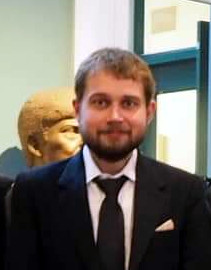
\includegraphics[width=2.5cm]{me.jpg}}} \end{picture}

\noindent \textbf{\biling{Birth date}{Fecha de nacimiento}}: 24/02/1989, \biling{USSR}{URSS} \\
\textbf{\biling{Citizenship}{Ciudadanía}}: \biling{Russian}{ruso}

{\color{RoyalBlue}\section*{\biling{ACADEMIC INTERESTS}{INTERESES ACADÉMICOS}}}

\biling{Algebraic geometry}{Geometría algebraica},
\biling{number theory}{teoría de números}.

\vspace{1em}

{\color{RoyalBlue}\section*{\biling{EDUCATION}{EDUCACIÓN}}}

\begin{itemize}
\item \textbf{2014--2018}: \textbf{\biling{University of Bordeaux}{Universidad de Burdeos}} (\biling{France}{Francia}),
  \textbf{\biling{Leiden University}{Universidad de Leiden}} (\biling{Netherlands}{Países Bajos}).

  \biling{ALGANT DOC Program}{Programa ALGANT DOC}, \biling{European Union scholarship}{beca de la Unión Europea}.

  \textbf{PhD \biling{in mathematics}{en matemáticas}}.

  \biling{Thesis}{Tesis} \biling{``}{<<}Zeta-values of arithmetic schemes at negative integers and Weil-étale cohomology\biling{''}{>>},\\
  \biling{supervised by}{dirigida por} Baptiste Morin (\biling{Bordeaux}{Burdeos}) \biling{and}{y} Bas Edixhoven (Leiden).

  \biling{Oficial defense}{Defensa oficial}: Leiden, \biling{December 10, 2018}{10 de diciembre de 2018}.

  \biling{Referees and examining committee}{Jurado}:
  P.~Cassou-Noguès (Université de Bordeaux),
  Ph.~Cassou-Noguès (Université de Bordeaux),
  D.~Holmes (Universiteit Leiden)
  R.~de Jeu (Vrije Universiteit Amsterdam),
  W.~van der Kallen (Universiteit Utrecht),
  H.~Lenstra (Universiteit Leiden),
  S.~Lichtenbaum (Brown University),
  N.~Ramachandran (University of Maryland),
  P.~Stevenhagen (Universiteit Leiden).

\item \textbf{2012--2014}: \textbf{\biling{University of Milan}{Universidad de Milán}} (\biling{Italy}{Italia}),
  \textbf{\biling{University of Bordeaux}{Universidad de Burdeos}} (\biling{France}{Francia}).

  \biling{ALGANT Master Program}{Programa ALGANT Master}, \biling{European Union scholarship}{beca de la Unión Europea}.

  \textbf{\biling{MSc in Mathematics}{Maestro en Ciencias con orientación en matemáticas}}.

  \biling{MSc thesis}{Tesis de maestría}
  \biling{on algebraic K theory}{sobre la teoría K algebraica},
  \biling{supervised by}{dirigida por} Boas Erez (\biling{Bordeaux}{Burdeos}).

\item \textbf{2010--2012}: \biling{University of the Russian Academy of Sciences}{Universidad de la Academia de Ciencias de Rusia},
  \biling{St. Petersburg}{San Petersburgo}, \biling{Department of Mathematics and Computer Science}{Facultad de matemáticas e informática}.

  \textbf{\biling{MSc in theoretical computer science}{Maestro en Ciencias con orientación en informática teórica}},
  diploma cum laude.

  \biling{Thesis advisor}{Director de tesis}: Dmitrii Pasechnik.

\item \textbf{2006--2010}: \biling{Lipetsk State University}{Universidad Estatal de Lipetsk}, \biling{Russia}{Rusia}.

  \textbf{\biling{BSc in computer science and software engineering}{Licenciado en ciencias de computación y programación}},
  diploma cum laude.
\end{itemize}

\pagebreak

{\color{RoyalBlue}\section*{\biling{POSITIONS}{POSICIONES}}}

\begin{itemize}
\item \textbf{\biling{October}{Octubre de} 2019 -- \biling{November}{noviembre de} 2020}:
  \textbf{Centro de Investigación en Matemáticas (CIMAT)},
  Guanajuato, \biling{Mexico}{México}, \textbf{\biling{visiting researcher}{investigador invitado}}.
  
  \biling{Hosts}{Anfitriones}: Xavier Gómez Mont, Pedro Luis del Ángel.

\item \textbf{\biling{February}{Febrero de} 2018 -- \biling{August}{agosto de} 2019}:
  \biling{University of}{Universidad de} El~Salvador,
  \biling{Natural Sciences Faculty, School of Mathematics}{Facultad de Ciencias Naturales, Escuela de Matemáticas},
  \textbf{\biling{visiting professor}{profesor invitado}}.

  \biling{Colaboration with the Ministry of Education of}{Colaboración con el Ministerio de Educación de} El~Salvador,
  \biling{to support the master program in mathematics}{con el fin de apoyar el programa de maestría en matemáticas}.
  \biling{Lectures for master and bachelor students}{Clases para estudiantes de maestría y licenciatura},
  \biling{editing of}{redacción de}
  \href{https://cadadr.org/san-salvador/}{\biling{teaching materials}{materiales didácticos}}, etc.
\end{itemize}

{\color{RoyalBlue}\section*{\biling{TALKS}{CONFERENCIAS}}}

\begin{itemize}
\item \textbf{\biling{February}{Febrero de} 2020}: Coloquio Oaxaqueño de Matemáticas,
  IMUNAM, Oaxaca.

\item \textbf{\biling{December}{Diciembre de} 2019}: First IMSA Conference,
  IMUNAM/CINVESTAV, \biling{Mexico City}{CDMX}.

\item \textbf{\biling{November}{Noviembre de} 2019}: Universidad Autónoma de Zacatecas
  (\biling{three talks}{tres conferencias}).

\item \textbf{\biling{October}{Octubre de} 2019}: \biling{XIII Algebra and Topology Workshop}{XIII Taller de Álgebra y Topología},
  IMUNAM, Cuernavaca.

\item \textbf{\biling{October}{Octubre de} 2019}: \biling{Seminario de geometría algebraica}{Algebraic geometry seminar},
  CIMAT, Guanajuato.

\item \textbf{\biling{May}{Mayo de} 2019}: \biling{Samuel Gitler Conference}{Conferencias Samuel Gitler},
  CINVESTAV, \biling{Mexico City}{CDMX}.

\item \textbf{\biling{December}{Diciembre de} 2017}:
  Algebra, geometry and number theory seminar, Leiden.
\end{itemize}

{\color{RoyalBlue}\section*{\biling{PUBLICATIONS}{PUBLICACIONES}}}

\begin{itemize}
\item Alexey Beshenov, Margaret Bilu, Yuri Bilu, Purusottam Rath,
  \emph{Rational points on analytic varieties},
  EMS Surv. Math. Sci. 2 (2015), no. 1, 109–130.

  \url{https://doi.org/10.4171/EMSS/10}

\item Alexey Beshenov,
  \emph{Zeta-values of arithmetic schemes at negative integers and Weil-étale cohomology},
  \biling{PhD thesis}{tesis doctoral}, Leiden University, December 2018.

  \url{https://openaccess.leidenuniv.nl/handle/1887/68224}

\item Alexey Beshenov,
  \emph{Weil-étale cohomology for arbitrary arithmetic schemes and $n < 0$.
    Part I: Construction of Weil-étale complexes},
  2020, preprint (arXiv:2012.11034).

  \url{https://arxiv.org/abs/2012.11034}

\item Alexey Beshenov,
  \emph{Weil-étale cohomology for arbitrary arithmetic schemes and $n < 0$.
    Part II: The special value conjecture},
  \biling{in preparation}{en preparación}.
\end{itemize}

\pagebreak

{\color{RoyalBlue}\section*{\biling{TEACHING EXPERIENCE}{EXPERIENCIA DOCENTE}}}

\noindent\textbf{\biling{One-semester courses}{Cursos semestrales}}

\vspace{0.5em}

\begin{itemize}
\item \textbf{\biling{Fall}{Otoño de} 2020}:
  \href{https://cadadr.org/cimat-tna/}{\textbf{\biling{Algebraic number theory}{Teoría de números algebraicos}}},
  \biling{Master program in pure mathematics}{maestría en matemáticas básicas},
  CIMAT, Guanajuato.

\item \textbf{\biling{Spring}{Primavera de} 2019}:
  \href{https://cadadr.org/san-salvador/2019-groebner/}{\textbf{\biling{Computational commutative algebra (Gröbner bases)}{Álgebra conmutativa computacional (bases de Gröbner)}}}
  \biling{for master students}{para la maestría}, \UES.

\item \textbf{\biling{Spring}{Primavera de} 2019}:
  \href{https://cadadr.org/san-salvador/2019-algebra/}{\textbf{\biling{Algebra}{Álgebra} I (\biling{rings and groups}{anillos y grupos})}}
  \biling{for undergraduate students}{para la licenciatura}, \UES.

\item \textbf{\biling{Spring}{Primavera de} 2018}:
  \href{https://cadadr.org/san-salvador/2018-08-algebra-conmutativa/}{\textbf{\biling{Commutative algebra}{Álgebra conmutativa}}}
  \biling{for master students}{para la maestría}, \UES.

\item \textbf{\biling{Fall}{Otoño de} 2018}:
  \href{https://cadadr.org/san-salvador/2018-algebra/}{\textbf{\biling{Algebra}{Álgebra} II (\biling{rings and fields}{anillos y campos})}}
  \biling{for undergraduate students}{para la licenciatura}, \UES.

\item \textbf{\biling{Spring}{Primavera de} 2018}:
  \href{https://cadadr.org/san-salvador/2018-algebra/}{\textbf{\biling{Algebra}{Álgebra} I (\biling{groups}{grupos})}}
  \biling{for undergraduate students}{para la licenciatura}, \UES.
\end{itemize}

\noindent\textbf{\biling{Minicourses}{Minicursos}}

\begin{itemize}
\item \textbf{\biling{Fall}{Otoño de} 2019}:
  \href{https://cadadr.org/cimat-zeta/}{\textbf{\biling{Around arithmetic zeta functions}{En torno de las funciones zeta aritméticas}}},
  CIMAT, Guanajuato.

\item \textbf{\biling{August}{Agosto de} 2019}:
  \href{https://cadadr.org/san-salvador/2019-esquemas/}{\textbf{\biling{Scheme theory}{Teoría de esquemas}}}
  \biling{for master students}{para la maestría}, \UES.

\item \textbf{\biling{November}{Noviembre de} 2018}:
  \href{https://cadadr.org/san-salvador/2018-cp-tne/reciprocidad-cuadratica.pdf}{\textbf{\biling{Quadratic reciprocity law}{La ley de reciprocidad cuadrática}}}
  \biling{for undergraduate students}{para la licenciatura}, \UES.

\item \textbf{\biling{July}{Julio de} 2018}:
  \href{https://cadadr.org/san-salvador/2018-07-reciprocidad/reciprocidad.pdf}{\textbf{\biling{Reciprocity laws from Gauss to Artin}{Las leyes de reciprocidad de Gauss a Artin}}},
  \UES.

\item \textbf{\biling{June}{Junio de} 2018}:
  \href{https://cadadr.org/san-salvador/2018-06-categorias/}{\textbf{\biling{Category theory}{Teoría de categorías}}}
  \biling{for master students}{para la maestría}, \UES.

\item \textbf{\biling{April}{Abril de} 2018}:
  \href{https://cadadr.org/san-salvador/2018-04-numeros-p-adicos/}{\textbf{\biling{p-adic numbers}{Números p-ádicos}}}
  \biling{for master students}{para la maestría}, \UES.

\item \textbf{\biling{February}{Febrero de} 2018}:
  \href{https://cadadr.org/san-salvador/2017-02-bernoulli/}{\textbf{\biling{Bernoulli numbers}{Números de Bernoulli}}},
  \UES.

\item \textbf{\biling{August--september}{Agosto–septiembre de} 2016}:
  \href{https://cadadr.org/san-salvador/2016-08-homo/}{\textbf{\biling{Homological algebra}{Álgebra homológica}}},
  \UES.
\end{itemize}

{\color{RoyalBlue}\section*{\biling{LANGUAGES}{IDIOMAS}}}

\biling{Russian}{Ruso} (\biling{native}{nativo});
\biling{Spanish}{español},
\biling{English}{inglés} (\biling{fluent}{fluido});
\biling{French}{francés},
\biling{Italian}{italiano} (\biling{intermediate}{intermedio}).

\vspace{1em}

{\color{RoyalBlue}\section*{\biling{COMPUTER SKILLS}{CONOCIMIENTOS INFORMÁTICOS}}}

LaTeX,
\biling{programming}{programación},
\biling{computer algebra systems}{sistemas de álgebra computacional}:
PARI/GP,
Sage,
Macaulay2,
GAP4.

\vspace{1em}

{\color{RoyalBlue}\section*{\biling{REFERENCES}{REFERENCIAS}}}

\begin{itemize}
\item Baptiste Morin (Université de Bordeaux)
\item Xavier Gómez Mont (CIMAT)
\item Pedro Luis del Ángel (CIMAT)
\end{itemize}

\end{document}
